\documentclass{book}
\usepackage{url}
\usepackage{xcolor}
\usepackage{array}
\usepackage{graphicx}

% \usepackage[T1]{fontenc}
\usepackage{upquote}
\usepackage{textcomp}
\usepackage{hyperref}
\usepackage{csquotes}
\usepackage{tex4ht-styles}



\usepackage{glossaries}
\title{TeX4ht Documentation}

\author{by TeX4ht Project}

\begin{document}

\maketitle

% Don't introduce table of contents in the HTML mode, as it introduces another page
\ifdefined\HCode\else\tableofcontents\fi


\chapter{Introduction}


\begin{acknowledgements}
This work was supported with a financial support from \href{https://cstug.cz/}{CSTUG}.
\end{acknowledgements}

\chapter{Basic Tutorial}
\section{What is \TeX4ht?}\label{what-is-tex4ht}

\href{https://www.tug.org/tex4ht/}{\texttt{TeX4ht}} is a system that
converts LaTeX to various output formats, including \texttt{HTML},
\href{http://en.wikipedia.org/wiki/OpenDocument}{\texttt{ODT}},
\href{http://en.wikipedia.org/wiki/DocBook}{\texttt{DocBook}} or
\href{http://en.wikipedia.org/wiki/Text_Encoding_Initiative}{\texttt{TEI}}.
\texttt{HTML} and \texttt{ODT} formats are the most common and best-supported
conversion targets.

\texttt{TeX4ht} allows authors to convert \LaTeX\ input to 
several output formats, like \texttt{HTML} (for web pages) or
\texttt{ePub} (for ebooks and other applications).

\hypertarget{basic-usage}{%
\section{Basic Usage}\label{sec:tutorial-basic-usage}}

Conversion is invoked using the \makefourht\ command:

\begin{shellcommand}
$ make4ht filename.tex
\end{shellcommand}


Let us start with conversion of a simple \LaTeX\ file to HTML  
with the following \LaTeX\ file:

\texinput{examples/otherlang/babel.tex}

You can compile it using the following command:

\begin{shellcommand}
$ make4ht -lm draft filename.tex
\end{shellcommand}

The resulting HTML file contains the following code:

\htmlinput{examples/otherlang/babel-lua-body.html}

As you can see, multiple options can be joined for \makefourht.  The above invocation is equal to the following:

\begin{shellcommand}
$ make4ht -l -m draft filename.tex
\end{shellcommand}

You can also use the long options:

\begin{shellcommand}
$ make4ht --lua --mode draft filename.tex
\end{shellcommand}

What do these options mean? 

The option \shellcmd{--lua} tells \makefourht\  to use Lua\LaTeX\ as a
compilation engine. There is also an option \shellcmd{-x} (or \shellcmd{--xetex})
that allows the use of Xe\LaTeX\ for the compilation. If neither of these options
is used, the file will be converted with the default PDF\LaTeX\ engine.

For example, if we compile the sample file without the \shellcmd{-l} option, we would get
a different result:

\htmlinput{examples/otherlang/babel-body.html}

Notice that the accents in the \textit{ť} and \textit{ď} letters are detached from the base letters.
That is because \texfourht{} uses information about characters in the DVI file. Current \LaTeX{}
supports basic accented characters out of the box, but sometimes, they don't work as expected.


The option \shellcmd{--mode} sets the compilation mode. \makefourht\  has one built-in mode,
named \texttt{draft}. 
By default, \makefourht{}  compiles your \TeX{} file three times, to obtain the correct hyperlinks 
and other features that depend on auxilary files. The \texttt{draft} mode uses
only one compilation run, so it is much faster.



\makefourht\  converts \LaTeX\ file to a HTML 5 document. You can request
conversion to other formats using the \texttt{-f} option. For example,
to convert a document to the OpenDocument Format, use the following:

\begin{shellcommand}
$ make4ht -f odt filename.tex
\end{shellcommand}

More information about \makefourht and its command line options and other features can be found in
section \namerefpage{sec:make4ht-intro}.


\section{\texfourht\ Options}

The simplest way to change some aspects of the design is to use \texfourht{} options. They can be passed
as a first positional argument after filename to \makefourht:

\begin{shellcommand}
$ make4ht filename.tex "option1,option2"
\end{shellcommand}

For example, \texfourht{} produces one HTML file for a document, but each footnote is placed in a separate file.
If you have a large document, you may want to use a separate page for each chapter, with a list of footnotes
at the end of these chapters. You can use the following options: 

\begin{shellcommand}
$ make4ht filename.tex "3,sec-filename,fn-in"
\end{shellcommand}


There are other numeric options, each of them breaks document into separate HTML pages on a different sectioning level. Option 1 does not break pages at all, 2 at parts, 3 at chapters, 4 at sections, 5 at subsections, 6 at sub-subsections, and 7 at paragraphs. The \verb|sec-filename| option will produce HTML file names that are based on section titles, instead of their numbers. The \verb|fn-in| option prints footnotes at the end of each HTML page.

There are also options that change the handling of math. Normally, HTML elements are used for simple math, and pictures are used for more complex features, such as fractions or square roots. This usually does not look good, so what are other options?

Generally, it is best to use \mathml{}, as it supports correct vertical alignment for inline math, and the font size matches the surrounding text. Unfortunately, some web browsers do not support it yet. We can use MathJax to render math in these browsers. 

\begin{shellcommand}
$ make4ht filename.tex "mathml,mathjax"
\end{shellcommand}

On the other hand, if you want to use pictures for math exclusively, you can try the \option{pic-m} option, which requires pictures even for inline math. There are also similar options for equations and other math environments.

\begin{shellcommand}
$ make4ht filename.tex "pic-m,pic-equation"
\end{shellcommand}

The generated pictures are in the PNG format, which is raster and depends on the resolution on the device where the document is displayed. You may want to use vector SVG format instead, as it should produce better quality of pictures:

\begin{shellcommand}
$ make4ht filename.tex "pic-m,pic-equation,svg"
\end{shellcommand}

For more information on options, see chapter \namerefpage{chap:options}.

\section{\makefourht{} extensions}

\makefourht{} has an extension support. These extensions can modify various aspects of the conversion process, for example, post-process the generated files, cache images, or add support for Rmarkdown files.
Extensions can be enabled using the \verb|-f format_name+extension_name| option. 

For example, there is a \verb|preprocess_input| extension, which adds support for Markdown or Rtex documents. It can process a following 
Rmarkdown document:

\texinput{examples/otherlang/rmarkdownsample.Rmd}

Compile it using the following command:

\begin{shellcommand}
$ make4ht -f html5+preprocess_input sample.Rmd
\end{shellcommand}

It producess a following HTML file:

\htmlinput{examples/otherlang/rmarkdownsample-body.html}

If your document produces many pictures, the compilation can take a long time. To make it faster, you can use the \verb|dvisvgm_hashes| extension. It caches the SVG images
and creates them only for the changed math environments.

\begin{shellcommand}
$ make4ht -f html5+dvisvgm_hashes filename.tex "pic-m,pic-equation,svg"
\end{shellcommand}

\makefourht{} loads the \verb|common_domfilters| extension automatically. It fixes common issues in the generated HTML files using the LuaXML package. To disable extension
from loading, use \verb|-extension_name| syntax:


\begin{shellcommand}
$ make4ht -f html5-common_domfilters filename.tex
\end{shellcommand}

You can find a list of extensions in \href{https://www.kodymirus.cz/make4ht/make4ht-doc.html#extensions}{\makefourht{} documentation}.

\section{Configurations}
\label{sec:tutorial-configurations}

Most of the markup produced by \texfourht{} is configurable. Supported commands 
can be configured using the \texcommand{\Configure} command. We can also insert 
markup before and after environments, using \texcommand{\ConfigureEnv} command.

While it is possible to insert these commands directly to your document, it is better
to use a custom configuration file, as you would get a compilation error if you compiled 
document containing \texfourht{} commands directly by \LaTeX.

You can find more information about syntax and available commands in section \namerefpage{sec:private-configuration}.
Here, we will show some simple examples.

\subsection{The \cmd{Configure} command}



You may want to insert some custom HTML tags. It is a bit more complicated for
\LaTeX commands, but it is easy for environments. You can configure the code that is 
inserted before and after environment using the \texcommand{\ConfigureEnv} command.
It has a following syntax:

\begin{texsource}
\ConfigureEnv{<environment name>}{before env}{after env}
{before-list}{after-list}
\end{texsource}

We can ignore the arguments \texttt{before-list} and \texttt{after-list}, as they
are used only for list like environments, such as \texttt{itemize}. So we just need to






But beware of the following situation:

\begin{texsource}
Hello world.
\begin{someenv}
Just start some environment.

But run it through several paragraphs
\end{someenv}
\end{texsource}

say that we insert
\htmlcommand{<div class="someenv">} and
\htmlcommand{</div>} tags around  the \texttt{someenv}
environment. By default this may produce following structure:

\begin{htmlsource}
<p>Hello world.
<div class="someenv">Just start some environment.
</p>

<p>But run it through several paragraphs
</div></p>
\end{htmlsource}

as you can see, generated html code is incorrect, as opening and closing
\htmlcommand{<div>} tags have different parent elements. \texttt{someenv} environment can
be configured to close current paragraph, but it may be not what you
want.

Best way to prevent tag mismatch may be something like:

\begin{texsource}
Hello world.
\begin{someenv}
Just start some environment.
\end{someenv}

\begin{someenv}
But run it through several paragraphs
\end{someenv}
\end{texsource}

and with \texttt{make4ht}

\begin{shellcommand}
make4ht sample1
\end{shellcommand}

lets look on text part generated by \texttt{htlatex}:

\begin{htmlsource}
<!--l. 6--><p class="noindent" >P&#x0159;íli&#353; &#382;lu&#x0165;ou&#x010D;k&#x00FD; k&#x016F;&#x0148; úp&#x011B;l <span 
class="ecti-1000">&#x010F;</span><span 
class="ecti-1000">ábelsk</span><span 
class="ecti-1000">é </span>ódy. Some text in English
\end{htmlsource}

and by \texttt{make4ht}:

\begin{htmlsource}
<!--l. 6--><p class="noindent" >P&#x0159;íli&#353; &#382;lu&#x0165;ou&#x010D;k&#x00FD; k&#x016F;&#x0148; úp&#x011B;l <span 
class="ecti-1000">&#x010F;</span><span 
class="ecti-1000">ábelsk</span><span 
class="ecti-1000">é </span>ódy. Some text in English
</p> 
\end{htmlsource}

only difference is missing \texttt{\textless{}/p\textgreater{}} tag in
output of \texttt{htlatex}, because \texttt{html\ 4.01} is produced by
\texttt{htlatex} by default. \texttt{make4ht} on the other hand produces
\texttt{xhtml} by default, so closing tag must be presented.

To get \texttt{xhtml} output from \texttt{htlatex}, use
\texttt{tex4ht.sty} option \texttt{xhtml}. This option must be first
option in the option list passed to \texttt{tex4ht.sty}. Value of the
first option must be either \texttt{html}, \texttt{xhtml} or name of
custom config file. We will cover these config files later, as they are
key component in customization of \texttt{TeX4ht} output.

So in order to get same output as from \texttt{make4ht}, we must use
following command:

\begin{shellcommand}
htlatex sample1 xhtml
\end{shellcommand}

Now we should get rid of ugly entities which encode accented letters.
This is somewhat ugly with \texttt{htlatex}:

\begin{shellcommand}
htlatex sample1 "xhtml,charset=utf-8" " -cunihtf -utf8"
\end{shellcommand}

\texttt{charset=utf-8} produces meta element which declares document to
be in \texttt{utf-8} encoding. Important are two options for
\texttt{tex4ht} command, \texttt{-c} and \texttt{-utf8}.

ToDo: add description of process of conversion from \texttt{htf} fonts
to utf8 using unicode.4hf. It is directed from \texttt{tex4ht.env} file.

With \texttt{make4ht}, situation is easier, as all we need to do is to
add \texttt{-u} option:

\begin{shellcommand}
make4ht -u sample1.tex
\end{shellcommand}

resulting file:

\begin{htmlsource}
<!--l. 6--><p class="noindent" >Příliš žluťoučký kůň úpěl <span 
class="ecti-1000">ď</span><span 
class="ecti-1000">ábelsk</span><span 
class="ecti-1000">é </span>ódy. Some text in English
</p> 
\end{htmlsource}

Entities are gone, but other persists. What we see is caused by a bug in
\texttt{tex4ht} command. It decorates text which is set in non-default
font with \texttt{\textless{}span\textgreater{}} elements. Unfortunately
it doesn't play well with accented letters as we can see. This has easy
solution, fortunately. We just need to dive into \texttt{TeX4ht}
configuration. Yay!

\hypertarget{configurations}{%
\section{Configurations}\label{configurations}}

We already saw that we can use command line options to configure the
output. For full list of options for \texttt{tex4ht.sty}, see an
\href{http://www.cvr.cc/?p=504}{article on CVR's blog}. These options
mainly influence appearance or math, footnotes, tables, etc. Note that
these options aren't fixed set, anyone can add new options and not all
options are supported in each output format supported by
\texttt{tex4ht}. Generally these options work with \texttt{html} (and
\texttt{xhtml}) output.

Other option is to use custom config file (\texttt{.cfg}). This is a TeX
file with some basic structure:

\begin{texsource}
 optional stuff like requiring LaTeX packages etc
 ...
 \Preamble{xhtml,tex4ht.sty options}
 ...
 TeX4ht configurations
 ...
 \begin{document} 
 ...
 more TeX4ht configurations
 ...
 \EndPreamble
\end{texsource}

Most important command for configuring is
\texttt{\textbackslash{}Configure}. This command has variable number of
arguments, in the simplest form it does have two arguments:
\texttt{\textbackslash{}Configure\{configname\}\{insert\ for\ a\ first\ hook\}}.

At this place we should talk about hooks. In order to insert html tags,
LaTeX macros are redefined and in the definitions special hooks are
inserted. These hooks are declared with
\texttt{\textbackslash{}NewConfigure\{configname\}\{number\ of\ hooks\}}
in special file named as redefined package name with suffix
\texttt{.4ht}. These hooks are then seeded in configure files for
particular output formats, or in the \texttt{.cfg} file.

To illustrate that, we can show some simple example. Lets say we have
simple package \texttt{hello.sty}:

\begin{texsource}
\ProvidesPackage{hello} 
\newcommand\hello{\textbf{hello world}}
\endinput
\end{texsource}

we can provide hooks in file named \texttt{hello.4ht}. Say we just want
to insert tags at beginning and at end of \texttt{\textbackslash{}hello}
command:

\begin{texsource}
% provide configure for \hello command. we can choose any name
% but most convenient is to name hooks after redefined command
% we declare two hooks, to be inserted before and after the command
\NewConfigure{hello}{2}
% now we need to redefine \hello. save it to tmp command
\let\tmp:hello\hello
% note that `:` can be part of command name in `.4ht` files. 
% now insert the hooks. they are named as \a:hook, \b:hook, ..., \h:hook
% depending on how many hooks were declared
\renewcommand\hello{\a:hello\tmp:hello\b:hello} 
\end{texsource}

because we want to surround contents produced by
\texttt{\textbackslash{}hello} with tags, we need to declare two hooks.
This is the most usual case for normal commands which just produce some
text. Old contents of macro are saved in temporary macro and then
command is redefined to insert hooks and original contents stored in
temporary macro.

Now we can change our sample to use \texttt{hello} package:

\begin{texsource}
\documentclass{article}
\usepackage[english,czech]{babel} 
\usepackage[T1]{fontenc}
\usepackage[utf8]{inputenc} 
\usepackage{hello}
\begin{document} Příliš žluťoučký kůň úpěl \textit{ďábelské} ódy.
\begin{otherlanguage}{english} Some text in English, \hello
\end{otherlanguage} 
\end{document}
\end{texsource}

we haven't provided any configurations for \texttt{hello} yet, but you
can see that text \texttt{hello\ world} is in \textbf{bold} font anyway.
This is the same case as \texttt{\textbackslash{}textit} which is
converted as \emph{italic}. Basic font styles are inserted by
\texttt{tex4ht} command during extraction of text from \texttt{dvi} to a
output format. So it is the right time to finally show how to configure
both \texttt{textit} and \texttt{hello} to produce some better tags than
they provide by default.

Basic structure of a config file has been shown before, so now we will
just add basic configurations for \texttt{\textbackslash{}textit} and
\texttt{\textbackslash{}hello}:

\begin{texsource}
\Preamble{xhtml}
\Configure{textit}{\HCode{<span class="textit">}}{\HCode{</span>}}
\Configure{hello}{\HCode{<span class="hello">}}{\HCode{</span>}}
\Css{.textit{font-style:italic;}}
\Css{.hello{font-weight:bold;}}
\begin{document}
\EndPreamble
\end{texsource}

For documentation of default configurations, see
\href{http://michal-h21.github.io/src4ht/tex4ht-info.html}{TeX4ht info},
most useful are
\href{http://michal-h21.github.io/src4ht/tex4ht-infose2.html}{LaTeX} and
\href{http://michal-h21.github.io/src4ht/tex4ht-infose1.html}{TeX4ht}
sections. Documentation for basic font commands such as
\texttt{\textbackslash{}textit} or \texttt{\textbackslash{}textbf} is
provided in
\href{http://michal-h21.github.io/src4ht/tex4ht-infose2.html}{LaTeX}
section. We can see that configuration takes two parameters, insertion
before and after content. Same situation is with \texttt{hello}
configuration we defined earlier, hooks are inserted before and after
the content.

To insert \texttt{html} tags, we need to use
\texttt{\textbackslash{}HCode} commands, special characters such as
\texttt{\textless{}},\texttt{\textgreater{}} or \texttt{\&} are escaped
otherwise. In our example we insert \texttt{span} elements with some
\texttt{class} attribute to distinguish them. Because these classes
doesn't have any visual appearance by default, we use
\texttt{\textbackslash{}Css} commands to add some styling. Yes, you need
to know both \texttt{html} and \texttt{css} to effectively configure
\texttt{TeX4ht}!

If we look at \texttt{html} output now, we can see that things don't
look much better than initially:

\begin{htmlsource}
<!--l. 6--><p class="noindent" >Příliš žluťoučký kůň úpěl <span class="textit"><span 
class="ecti-1000">ď</span><span 
class="ecti-1000">ábelsk</span><span 
class="ecti-1000">é</span></span> ódy. Some text in English, <span class="hello"><span 
class="ecbx-1000">hello world</span></span>
</p> 
\end{htmlsource}

our new tags were inserted, but unnecessary elements inserted by
\texttt{tex4ht} processor are still present. Fortunately, we can
suppress insertion of these elements with
\texttt{\textbackslash{}NoFonts} command, and later enable again with
\texttt{\textbackslash{}EndNoFonts}. We can also use \texttt{tex4ht.sty}
option \texttt{NoFonts}, which will suppress font processing in whole
document, but you should use this with caution, as it may have some side
effects.

Let's take a look how would out configurations look with
\texttt{\textbackslash{}NoFonts} command:

\begin{texsource}
\Preamble{xhtml}
\Configure{textit}{\HCode{<span class="textit">}\NoFonts}
{\EndNoFonts\HCode{</span>}}
\Configure{hello}{\HCode{<span class="hello">}\NoFonts}
{\EndNoFonts\HCode{</span>}}
\Css{.textit{font-style:italic;}}
\Css{.hello{font-weight:bold;}}
\begin{document}
\EndPreamble
\end{texsource}

the output now looks much better:

\begin{htmlsource}
<!--l. 6--><p class="noindent" >Příliš žluťoučký kůň úpěl <span class="textit">ďábelské</span> ódy. Some text in English, <span class="hello">hello world</span>
</p> 
\end{htmlsource}

It may seems that we can be happy at this point, but things aren't as
easy as we may hope, because we haven't talked about one thing:

\hypertarget{paragraphs}{%
\section{Paragraphs}\label{paragraphs}}

What if we add some more paragraphs in English to our sample file?

\begin{texsource}
\documentclass{article}
\usepackage[english,czech]{babel} 
\usepackage[T1]{fontenc}
\usepackage[utf8]{inputenc} 
\usepackage{hello}
\begin{document} Příliš žluťoučký kůň úpěl \textit{ďábelské} ódy.
\begin{otherlanguage}{english} Some text in English, \hello
\end{otherlanguage} 

\begin{otherlanguage}{english} 

\textit{What will do} \verb|\textit| at the beginning of paragraph?

And also, what about configuration for \verb|otherlanguage| environment?

\end{otherlanguage}

\end{document}
\end{texsource}

What if we want to insert elements with \texttt{lang} attribute to
specify language of text in the \texttt{html}. It might be useful from
semantic point of view, we can also enable hyphenation in the
\texttt{css} and it works only when correct languages are marked in the
source.

This exercise will be little bit more difficult

\chapter{How to}

\section{Change design}
\subsection{Basics}

By default, \texfourht\ separates paragraphs by spaces. If you want to use text indenting instead, try the \option{p-indent} option.

\subsection{CSS}
\subsection{Web fonts}

It is easy to change fonts in the web pages using CSS, but if you want to use
actual font files for the distribution, for example in an Epub file, \texfourht
provides following configurations. This example shows how to use OTF files
for the EB Garamond font. 

\begin{texsource}
% define font family. The first argument is family name
% that can be used in CSS font-family rule
% second argument is the family name declared by the font
\Configure{FontFamily}{rmfamily}{EB Garamond}
% declare font filenames for particular font styles. 
% the font files must be placed in the location that is
% declared.
% these four font styles are supported
\Configure{NormalFont}{EBGaramond-Regular.otf}
\Configure{ItalicFont}{EBGaramond-Italic.otf}
\Configure{BoldFont}{EBGaramond-Bold.otf}
\Configure{BoldItalicFont}{EBGaramond-BoldItalic.otf}
% use CSS to use the declared font family in the document
% serif is used as a fallback
\Css{body{font-family: "rmfamily", serif;}}
\end{texsource}


\section{Math}

\subsection{MathJax}


\subsection{MathML}
\subsection{Subscripts and superscripts}
% info about super and subscripts with MathML
% https://tex.stackexchange.com/q/518839/2891

Subscript and superscript support in \texfourht\ is a bit complicated. The
catcodes of \texcommand{_} and \texcommand{^} characters are changed and they are
active characters instead. This is necessary in order to insert the markup tags
for these structures. One consequence of this is that you need to use a correct grouping
for content that should be affected by these operators.
For example, instead of 

\begin{texsource}
$A_\mathit{...}$
\end{texsource}

use the following, with added group around the \texcommand{\mathit} command:

\begin{texsource}
$A_{\mathit{...}}$
\end{texsource}

If you define custom commands in the document preamble, use \texcommand{\sp}
and \texcommand{\sb} instead of \texcommand{^} and \texcommand{_}.

For example:

\begin{texsource}
\newcommand \coeffX [4][X]{\mathbf{#1}_{{#2},{#3}}(#4)}
\end{texsource}

should become:

\begin{texsource}
\newcommand\coeffX [4][X]{{\mathbf{#1}}\sb{#2,#3}(#4)}
\end{texsource}

Sometimes, it is not possible to change the source files. In this situation, you 
can pre-process the source using custom script that reads the original file, fixes the code
and then pipes the modified output to \shellcmd{make4ht}.

For example, you may want to change this input:

\begin{texsource}
$k'^4_{i}$
\end{texsource}

to the correct form:

\begin{texsource}
$k^{\prime 4}_{i}$
\end{texsource}

This, and other common issues, can be done using the following Lua script:

\begin{luasource}
for line in io.lines() do
  -- fix primes
  line = line:gsub([[%'%^(.-)%_]], [[^{\prime %1}_]])
  -- fix \mathrm{hello}^2
  line = line:gsub([[(\[a-zA-Z]-)(%b{})([%^%_])]], [[{%1%2}%3]])
  -- fix x_\mathrm{hello}
  line = line:gsub([[([%_%^])(\[a-zA-Z]-)(%b{})]], "%1{%2%3}")
  -- fix 10^2
  line = line:gsub("([%d])([%_%^])", "{%1}%2")
  -- fix {}_x
  line = line:gsub("{}([%_%^])", "{\\HCode{}}%1")
  print(line)
end
\end{luasource}

It uses Lua version of regular expressions to find the code we want to fix.
The command to execute it could be:

\begin{shellcommand}
texlua filter.lua < sample.tex | make4ht -j sample - "mathml,mathjax"
\end{shellcommand}

The \shellcmd{-j} option is used to name the output file, which is necessary
because the input comes from a pipe. The dash used in the place of filename
tells \shellcmd{make4ht} to read input from the standard input.

We use \shellcmd{MathJax} to render \mathml, as \mathml\ is not supported by
all browsers. 

\subsection{MathJax Node}


\section{Graphics}
\subsection{Include graphics (svg,pdf)}
\subsection{Change image size and resolution}
You can use \texcommand{\Configure{Gin-dim}} command to change the way how image dimensions
are calculated. By default, \texfourht\ relies on information about image
dimensions provided by the Graphics package. If you use explicit dimensions
(like \texcommand{width=0.5\textwidth}), the actual dimension calculated by \TeX\ is used.

One problem is that if you set only one dimension, for example width, the other
dimension will be set to the same value. You usually don't want this, unless
your image is a square. To get the correct value for all dimensions, Graphics
uses a \verb|.xbb| file for image. It can be created using the following command:

\begin{shellcommand}
ebb -x *.jpg
\end{shellcommand}

Run analogous command for every other supported image format you use. This will
ensure that correct values are used for implicitly calculated dimensions.

\subsection{Use relative size for images}

The following configuration file example can be used to get image dimensions
relative to the original page width. Thanks to the \LaTeX\ 3 project, we can 
use the \package{l3fp} package to calculate the image dimensions in percents. 

\begin{texsource}
\Preamble{xhtml}
\makeatletter
\ExplSyntaxOn
\Configure{Gin-dim}
{style="width:\fp_eval:n{round(\Gin@req@width/\textwidth*100,2)}\%"}
\ExplSyntaxOff
\makeatother
\begin{document}
\EndPreamble
\end{texsource}

In this configuration, we divide the image width passed to
\texcommand{\includegraphics} by the document text width. 
This portion is then multiplied and rounded to get the correct percent value.
The calculated value is used in the \verb|style| attribute of the generated \verb|<img>| element.
The \package{l3fp} command \texcommand{\fp_eval:n} is used for the calculation. 
\LaTeX\ 3 is part of \LaTeX\ kernel, so we don't need to require packages that it provides.

The following example code:

\begin{texsource}

\includegraphics[width=0.5\textwidth]{example-image.png}
\end{texsource}

produces following HTML code:

\begin{htmlsource}
<img style='width:50%' alt='PIC' src='example-image.png' />
\end{htmlsource}

To disable setting of the image dimensions in HTML code completely
use the following configuration:

\begin{texsource}
\Preamble{xhtml}
\Configure{Gin-dim}{}
\Css{img {
    max-width: 100\%;
    height: auto;
}}
\begin{document}
\EndPreamble
\end{texsource}

This configuration uses CSS to set the maximum image dimension. This ensures that
the image is donwsized on devices smaller than is the actual image size.


\subsection{Change image \texttt{alt} attribute}

By default, \package{Graphicx} package doesn't support the attribute that could
be used to insert alternative text that describe the image. This is necessary
for the accessibility purposes.

We can define a new attribute for \texcommand{\includegraphics} command, named
\texttt{alt}, for example. Here is a sample file that shows how to do that:

\texinput{examples/imagealt/sample.tex}

The \texcommand{\define@key{Gin}{alt}{}} command defines a dummy command that
is used by regular \LaTeX. We need to redefine this key for \texfourht, so it uses the
configuration that can specify the image alternative text, \configuration{GraphicsAlt}.

\texinput{examples/imagealt/mycfg.cfg} 

The resulting HTML file now contains image with the \texttt{alt} attribute:

\htmlinput{examples/imagealt/sample-body.html}


\section{Plain \TeX}

\texfourht\ supports Plain \TeX, but it can be a bit tricky. In general, you
will have to provide configurations to get good markup for your custom
commands. You will also need to add few commands to your source file: 

\begin{texsource}
%!TEX TS-program = tex
\input plain-4ht.tex
\document
Hello world
\enddocument
\end{texsource}

The first line contains magic comment that tells \texttt{make4ht} to use Plain
\TeX\ instead of \LaTeX for the compilation. \texcommand{\document} and \texcommand{\enddocument}
commands are important, because they are crucial for correct execution of \texfourht.

They are declared in the \texttt{plain-4ht.tex} file:

\begin{texsource}
\def\documentstyle#1{}
\documentstyle{tex4ht}
\csname tex4ht\endcsname
\def\document{}
\def\enddocument{\csname bye\endcsname}
\end{texsource}

In the PDF mode, these commands will do nothing, except for execution of the \texcommand{\bye} command.

The document can be compiled using:

\begin{shellcommand}
make4ht -f html5+detect_engine filename.tex
\end{shellcommand}

The \verb|-f html5+detect_engine| requires the \verb|detect_engine| extension,
which uses the magic command in the source file to determine which \TeX\ engine
to use. It is necessary for the correct Plain \TeX\ support.


\section{Blogging}

\section{Work with external commands}
\subsection{Indexing}
\subsection{Bibliographies}
\subsection{R}
\subsection{Markdown}
\subsection{PythonTeX}


\chapter{Calling Commands}
The conversion process used by \texfourht\ involves several tools
(see section \ref{sec:overview}, \nameref{sec:overview} for details). 


We provide a build script, called \shellcmd{make4ht}, which simplifies the 
process.


\section{\texttt{make4ht} Build System}
\label{sec:make4ht-intro}

The conversion command loads a script which takes on itself to invoke the
different steps of the process, without user intervention. The command assumes
the form:

\begin{shellcommand}
make4ht [make4ht options] filename.tex "options1" "option2" "options3" "options4"
\end{shellcommand}

The first set of options is for the tex4ht.sty and *.4ht style files, the
second set is for the tex4ht post-processor, the third for the t4ht
post-processor, and the last one is for the \LaTeX\ compiler. 

These options are optional.

The basic invokation of make4ht looks like this:

\begin{shellcommand}
make4ht filename.tex
\end{shellcommand}

This command requests a translation according to the default conditions, which are set to produce HTML 5 document.

\begin{shellcommand}
make4ht filename.tex "2,info"
\end{shellcommand}

This command specifies some options for tex4ht.sty. The "2" option requests a
break up of the output into separate web pages, in accordance to the two top
sectioning levels of the document.

The \texttt{info} option requests inclusion of documentation of basic configurations to the \texttt{filename.log} file.
You can open this file using a text editor to read this information.

Information about additional options can be found in the \namerefpage{sec:texfouhtoptions} section.



\begin{shellcommand}
make4ht -c foo.cfg filename "frames" "" "-p"
\end{shellcommand}

This command requests LaTeX to load a \nameref{sec:private-configuration}, named
foo.cfg, using the \texttt{-c} make4ht option. The \texttt{frames} option
requires placing of the content and table of contents in separate frames. In
addition, it asks the \shellcmd{t4ht} command not to produce bitmaps for pictures using the \shellcmd{-p} option.

\section{\makefourht{} Options}


\begin{shellcommand}
-a,--loglevel (default status) Set log level.
possible values: debug, info, status, warning, error, fatal
-b,--backend (default tex4ht) Backend used for xml generation. 
possible values: tex4ht or lua4ht
-c,--config (default xhtml) Custom config file
-d,--output-dir (default nil)  Output directory
-e,--build-file (default nil)  If build file is different than `filename`.mk4
-f,--format  (default html5)  Output file format
-h,--help  Display this message
-j,--jobname (default nil)  Set the jobname
-l,--lua  Use lualatex for document compilation
-m,--mode (default default) Switch which can be used in the makefile 
-n,--no-tex4ht Disable dvi file processing with the tex4ht command
-s,--shell-escape Enables running external programs from LaTeX
-u,--utf8  [obsolete] The document is generated in UTF8 encoding by default
-v,--version  Display version number
-x,--xetex Use xelatex for document compilation
\end{shellcommand}

\subsection{Terminal Output}

\makefourht\ hides the terminal output by default. It shows only errors and warnings.
It doesn't always show the correct error context. In such cases, try the \shellcmd{-a debug} option.
It is also recommended to use output of this option for \TeX4ht bug reports.

\begin{shellcommand}
$ make4ht -a debug -m draft buggy.tex
\end{shellcommand}

\subsection{Output Directory}

To copy generated files to a different directoy, use the \shellcmd{-d path} option. The passed path
can be absolute or relative to the current directory. It also doesn't need to exist, \makefourht{}
will create it if necessary.

\begin{shellcommand}
$ make4ht -d outdir filename.tex
\end{shellcommand}

Note that this option doesn't remove any files from the current directory. If you want to remove the temporary
files, use the \shellcmd{-m clean} option:

\begin{shellcommand}
$ make4ht -m clean filename.tex
\end{shellcommand}


\section{Overview of the Translation Process}\label{sec:overview}


The translation of a LaTeX source file into HTML involves loading of
the \texttt{tex4ht.sty} package. It watches loaded packages, and loads
corresponding configuration files, named as \texcommand{<pkgname>.4ht}. 
These configuration files patches commands provided by the packages, and
insert special hooks, which are later filled with XML code for the output format.

To ensure that all packages are processed, \texttt{tex4ht.sty} needs to be 
loaded early, ideally before \texcommand{\documentclass}.

Result of the \LaTeX{} run is a DVI file that contain document text and 
special instructions with XML code, or with requests for pictures. 
This file is then processed by the \shellcmd{tex4ht} command. It generates
the output XML or HTML files and the IDV file, which is then used for 
pictures. 

The last command is \shellcmd{t4ht}. It generates pictures and CSS file.

Basic sequence of execution of these command is following:

\begin{shellcommand}
latex      x            (or ‘tex x’) 
latex      x 
latex      x 
tex4ht     x 
t4ht       x 
\end{shellcommand}

The three compilations with La(\TeX) are needed to ensure proper links. The approach is illustrated in the picture \ref{fig:process}. 

\begin{figure}
  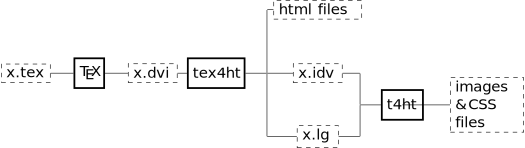
\includegraphics[width=\textwidth]{images/tex4ht_process/tex4ht_process}
  \caption{\texfourht\ process overview}
  \label{fig:process}
\end{figure}

\begin{description}
  \item[x.tex]

This is a source TeX/LaTeX/OtherTeX file that imports the style files tex4ht.sty and *.4ht. The style files define the features for the output.

\item[tex4ht]

The output of \TeX{} is a standard dvi file interleaved with special
instructions for the postprocessor \shellcmd{tex4ht} to use. The special
instructions come from implicit and explicit requests made in the source file
through commands of \texfourht.

The utility tex4ht translates the dvi code into standard text, while obeying
the requests it gets from the special instructions. The special instructions
may request the creation of files, insertion of html code, filtering of
pictures, and so forth.

In the extreme case that the source code contains no commands of \TeX4ht, it
gets the pure dvi code and it outputs (almost) plain text with no hypertext
elements in it.

The special (\texcommand{\special}) instructions seeded in the DVI code are not understood
by dvi processors other than those of \TeX4ht.

\item[x.idv]

This is a dvi file extracted from x.dvi, and it contains the pictures needed in
the html files.

\item[x.lg]

This is a log file listing the pictures of x.idv, the png files that should be
created, CSS information, and user directives introduced through the
‘\texcommand{\Needs{...}}’ command.

\item[t4ht]
This is an interpreter for executing the requests made in the x.lg script.

\end{description}

\subsection{make4ht extensions}\label{sec:make4ht-extensions}

\label{sec:calling-commands}
\chapter{Output Formats}
\chapter{\texfourht\ Options}

% the list of options has been copied from the CVR's blog
% http://cvr.cc/?p=504



Following is an incomplete list of options that can be passed to the \fourhtsty\ package.
These options can be used to modify the compilation process, for example to
select a \term{SVG} format for generated images, to request math environments
to be convert as images or to split sections as separate HTML pages. 

The options may be defined in the \fourhtfile\ files and may depend on the
output format, so it is not feasible to provide their full list. Most of the
following options work only in the \HTML\ output.

There are several ways how to pass the options to \texfourht. The
non-recommended way is to pass them as options to \fourhtsty\ using
\texcommand{\usepackage} command in the \TeX\ file. 

Better ways don't require modifications of the \TeX\ files.
It is possible to pass the options to the calling script, as an command line
argument next to the filename:
% it is run from the command line. These can also be provided as options when \texfourht
% package is loaded in a \LaTeX\ document with the default usepackage command or to
% the \verb|\Preamble| command in the custom config file

\begin{shellcommand}
make4ht filename.tex "fn-in"
\end{shellcommand}

For more information about calling scripts see the section \ref{sec:calling-commands}.

It is also possible to pass options in the \texcommand{\Preamble} command in a \cfgfile.

\begin{texsource}
\Preamble{fn-in}
...
\begin{document}
\EndPreamble
\end{texsource}



\section{List of options}

% \begin{tabular}{>{\ttfamily}p{8em} l} 
%   -css & to ignore CSS code, use command line option -css. \\
%   -xtpipes & to avoid xtpipes post-processing the output. This might be useful for docbook XML output.\\
%   0 & pagination shall be obtained through the option 0 or 1, at locations marked with PageBreak.\\
%   1, 2, 3, 4, 5, 6, 7& for automatic sectioning pagination (to break at various section levels), use the appropriate command line option 1, 2, 3, 4, 5, 6, 7.
\begingroup
\catcode`\#=11 \catcode`\^=11 \catcode`\_=11


\begin{description}

\item[-css] to ignore \css\ code, use command line option \verb=-css=.

\item[-xtpipes] to avoid \verb=xtpipes= post-processing the
  output. This might be useful for docbook \xml\ output.

  % \item[/bib]
  % \item[/obeylines]
  % \item[0.0]

\item[0] pagination shall be obtained through the option \verb=0= or
  \verb=1=, at locations marked with \verb=\PageBreak=.

\item[1, 2, 3, 4, 5, 6, 7] for automatic sectioning pagination (to
  break at various section levels), use the appropriate command line
  option \verb=1, 2, 3, 4,= \verb=5, 6, 7=.

\item[DOCTYPE] to request a \verb=DOCTYPE= declaration, use the
  command line option \verb=DOCTYPE=.

\item[Gin-dim] for key dimensions of the graphic, try this option.

\item[Gin-dim+] for key dimensions when the bounding box is not
  available.

\item[NoFonts] to ignore \css\ font decoration.

\item[PMath] Option to choose positioned math. Example: 
  \verb=\def\({\PMath$}=;\allowbreak \verb=\def\){$\EndPMath}=;
  \verb=\def\[{\PMath$$}=; \verb=\def\]{$$\EndPMath}=.

\item[RL2LR] to reverse the direction of RL sentences.

%\item[ShowFont]

\item[TocLink] option to request links from the tables of contents.
  
\item[\textasciicircum 13] option for active superscript character.

\item[\_13] option for active subscript character.

\item[accent-] This option is available only together with
  \option{new-accents}. It produces pictures for some math accents.

%\item[base]

\item[bib-] for degraded bibliography friendlier for conversion to
  \verb=.doc=.

\item[bibtex2] Option \verb=bibtex2= requires compilation of
  \verb=\jobname j.aux= with bibtex.

%\item[broken-index]

\item[charset] for alternate character set, use the command line
  option \verb+charset="..."+ (e.g., \verb+charset="utf8"+).

%\item[core]

\item[css-in] the inline \css\ code will be extracted from the input of
  the previous compilation, so an extra compilaion might be needed for
  this option to make it effective.

\item[css2] for \css2 code.

% \item[css]
% \item[debug-]
% \item[debug]
% \item[draw]
% \item[dtd]

\item[early\textasciicircum] for default catcode of superscript in the
  \verb=\Preamble=.

\item[early\_] for default catcode of subscript in the
  \verb=\Preamble=.

%\item[edit]

\item[endnotes] for end notes instead of footnotes, use this option.

%\item[enum]

\item[enumerate+] for enumerated list elements that keep the list couter value. This
  will use the description list like \verb=<dt>...</dt>= for the list
  counter.

\item[enumerate-] for enumerated list element's \verb=<li>='s with
  value attributes, use this command line option. This will be an
  ordered list with the value of list counter provided as an attribute
  namely, \verb=value= of the \verb=<li>= element.

%\item[family]
\item[fancylogo] try to visually emulate \verb|\TeX| and \verb|\LaTeX| logos.

\item[fn-in] for inline footnotes use this option.

\item[fn-out] for offline footnotes.

\item[fonts] for tracing \latex\ font commands, use this command line
  option.

\item[fonts+] for marking of the base font, use this option.

\item[font] for adjusted font size, use the command line option
  \verb+font=...+ (e.g., font=-2).

\item[frames-] for frames support. \verb=frames= is also valid option
  for frames support.

\item[frames-fn] for content, \chfont{TOC}\ and footnotes in
  three frames.

\item[frames] for \chfont{TOC}\ and content in two frames.

%\item[fussy]

\item[gif] for bitmaps of pictures in \verb=.gif= format, use this
  option.

\item[graphics-] if the included graphics are of degraded quality, try
  the command line options \verb=graphics-num= or \verb=graphics-=.
  The \verb=num= should provide the density of pixels in the bitmaps
  (e.g., 110).

%\item[graphics-dim]

\item[hidden-ref] option to hide clickable index and bibliography
  references.

% \item[hooks++]
% \item[hooks+]
% \item[hooks]
% \item[hshow]
% \item[htm3]
% \item[htm4]
% \item[htm5]
% \item[htm]

\item[html+] for stricter \HTML\ code.

%\item[html]

\item[imgdir] for addressing images in a subdirectory, use the option
  \verb=\imgdir:.../=.

\item[image-maps] for \verb=image-maps= support.

\item[index] for \emph{n}-column index, use the command line option,
  \verb+index=n+ (e.g., index=2).

\item[info-oo] for extra tracing information while generating open
  office output.

\item[info] for extra information in the \verb=\jobname.log= file.

\item[java] for \verb=java=support.

\item[javahelp] for \verb=JavaHelp= output format, use this command
  line option.

\item[javascript] for \verb=javascript= support.

\item[jh-] for sources failing to produce \xml\ versions of \HTML, try
  this command line option.

%\item[jh1.0]

\item[jpg] for bitmaps of pictures in \verb=.jpg= format, use this
  option.

\item[li-] for enumerated list elements li's with value attributes.

\item[math-] option to use when sources fail to produce clean math
  code.

\item[mathjax] use \term{MathJax} for the math rendering.
%\item[mathaccent-]

\item[mathltx-] option to use when sources fail to produce clean
  \verb=mathltx= code.

\item[mathml-] option to use when sources fail to produce clean
  \mathml code.

\item[mathplayer] for \mathml\ on Internet Explorer + MathPlayer.

\item[minitoc\textless] for mini tocs immediately after the header use the
  command line option, \verb=minitoc<=.

\item[mouseover] for pop ups on mouse over.

\item[new-accents] alternative configurations for accented characters. 

\item[next] for linear cross-links of pages, use this option.

\item[nikud] for Hebrew vowels, use the command line option,
  \verb=nikud=.

\item[no-DOCTYPE] to remove \texttt{DOCTYPE}\space declaration from
  the output.

\item[no-VERSION] to remove \verb+<?xml version="..."?>+ processing
  instruction from the output.

\item[NoFonts] disable ht-fonts processing in the document.

% \item[no-align]
% \item[no-array]
% \item[no-bib]
% \item[no-cases]
\item[no-halign] suppress \texcommand{\halign} redefinition. It doesn't work with the \texcommand{tabular} environment.
% \item[no-matrix]
% \item[no-pmatrix]

\item[no\textasciicircum] for non-active \verb=^= (superscript), use the option
  \verb=no^=.

\item[no\_] for non-active \verb=_= (subscript command), use the
  command line option, \verb=no_=.

\item[no\_\textasciicircum] for both non-active superscript and subscript, use the
  option \verb=no_^=.

\item[nolayers] to remove overlays of slides, use this option.

\item[nominitoc] this will eliminate mini tables of contents from the
  output.

\item[notoc*] for tocs without \verb=*= entries, use this option. The
  \verb=notoc*= option is applicable only to pages that are
  automatically decomposed into separate web pages along section
  divides. It shall be used when \verb=\addcontentsline= instructions
  are present in the sources.

\item[obj-toc] for frames-like object based table of contents, use the
  command line option \verb=obj-toc=.

%\item[old-longtable]

\item[p-width] for width specifications of tabular \verb=p= entries,
  use this option.

\item[p-indent] for indented paragraphs, without blank spaces.

\item[pic-RL] for pictorial RL.

\item[pic-align] for pictorial align environment.

\item[pic-array] for pictorial array.

\item[pic-cases] for pictorial cases environment.

\item[pic-eqalign] for pictorial equalign environment.

\item[pic-eqnarray] for pictorial eqnarray.

\item[pic-equation] for pictorial equations.

\item[pic-fbox] for pictorial or bitmapped fbox'es.

\item[pic-framebox] for bitmap fameboxes.

\item[pic-longtable] for bitmapped longtable.

\item[pic-m+] for pictorial \verb=$...$= and \verb=$$...$$=
  environments with \latex\ alt, use the command line option
  \verb=pic-m+= (not safe).

\item[pic-m] for pictorial \verb=$...$= environments, use the command
  line option \verb=pic-m= (not recommended).

\item[pic-matrix] for pictorial matrix.

% \item[pic-tabbing']

% \item[pic-tabbing]

% \item[pic-table]

\item[pic-tabular] use this option for pictorial tabular.

\item[plain-] for scaled down implimentation.

% \item[pmathml-css]

% \item[pmathml]

% \item[postscript]

\item[prog-ref] for pointers to code files from root fragments, use
  the command line option \verb=prof-ref=. This is for debugging.

\item[refcaption] for links into captions, instead of flat heads, use
  this option.

\item[rl2lr] to reverse the direction of Hebrew words, use this
  option.

\item[sec-filename] for file names derived from section titles, use
  the command line option \verb=sec-filename=.

\item[sections+] for back links to table of contents, use this option.

% \item[sections-]
% \item[settabs-]
% \item[stackrel-]

\item[svg-] for external \svg\ files, try this option.

\item[svg-obj] same as above.

\item[svg] for dvi pictures in \verb=svg= format.

\item[svg-inline] same as the \option{svg}, but the \svg\ files are included in the document body.

\item[tab-eq] for tab-based layout of equation environment, use this
  option.

%\item[th4]

\item[trace-onmo] for mouseover tracing of compilation, use the
  command line option, \verb=trace-onmo=.

% \item[uni-emacspeak]
% \item[uni-html4]
% \item[uniaccents]
% \item[unicode]

% \item[url-]

\item[url-enc] for \chfont{URL}\space encoding within href, use this
  option.  \verb=\Configure{url-encoder}= can be used to fine tune
  encoding.

\item[url-il2-pl] for il2-pl \chfont{URL} encoding.

\item[ver] for vertically stacked frames. Effective when \verb=frames=
  option is requested.

% \item[verify+]
% \item[verify]

\item[xht] for file name extension, \verb=.xht=, use this command line
  option.

\item[xhtml] for \xml\ code, use the command line option, \verb=xml= or
  \verb=xhtml=.

\item[xml] See previous entry.

% \item[xmldtd]

\end{description}
\endgroup


\chapter{Configurations}
\section{Private Configuration Files}\label{sec:private-configuration}

The leading entry, in the first list of options of the \shellcmd{htlatex}-like
commands, can equal \option{html} or \option{xhtml}. If this is not the case,
the entry is assumed to be the name of a configuration file. The extension
‘cfg’ is assumed for names of configuration files that are listed without their
extension.

A configuration file should take the following form for LaTeX files.

\begin{texsource}
...early definitions...
\Preamble{options}
...definitions...
\begin{document}
...insertions into the header of the html file...
\EndPreamble
\end{texsource}

It is up to the user to decide the distribution of entries between the \texcommand{\Preamble} and the htlatex-like commands.

Example: The command \shellcmd{htlatex myfile "mycfg,2"} requests the
compilation of a file named \file{myfile.tex}, in the presence of a
configuration file named \file{mycfg.cfg}. The configuration file might have the
following content.

\begin{texsource}
\Preamble{html} 
\begin{document} 
  \Css{body { color : red; }} 
\EndPreamble 
\end{texsource}

Notes

\begin{itemize}
  \item Notice that for a LaTeX file the \texcommand{\begin{document}}
    instruction should be present both in the configuration file and the source
    file.

  \item Instructions defined within a source file may be redefined in a
    configuration file. Such a feature enables to keep source files intact for
    compilation to different formats by different tools.
\end{itemize}

For instance, a definition of the form \texcommand{\renewcommand\mycommand{...}} within a
configuration file provided for the following LaTeX source.

\begin{texsource}
\documentclass{...} 
\newcommand\mycommand{...} 
\begin{document} 
Use \mycommand{...} 
\end{document} 
\end{texsource}

\subsection{Configuration file management}

It is possible to reuse common \texfourht\ configurations used in several
configuration files.  They can be inserted in a custom LaTeX package, but there
is one important thing to be aware of. The configuration hooks are inserted to
the patched commands when the compilation reaches the  
\texcommand{\begin{document}} command, so configurations for these hooks
declared before the hook definition have no effect. It is necessary to include
them in the \texcommand{\AtBeginDocument} command.

Sample package, \file{commonconfigurations.sty}:

\begin{texsource}
\ProvidesPackage{commonconfigurations}
\AtBeginDocument{%
\Configure{@HEAD}
{\HCode{<meta name="test" content="test"/>\Hnewline}}
}
\endinput
\end{texsource}

It can be requested in a configuration file using \texcommand{\RequirePackage} command.

\begin{texsource}
\Preamble{xhtml}
\RequirePackage{commonconfigurations}
\begin{document}
\EndPreamble
\end{texsource}



\section{tex4ht Commands}
\subsection{Low-level \texfourht\ Commands}

\DocCommand{Configure}\marg{name}\marg{arg 1}\ldots\marg{arg n}

The \cmd{Configure} command declares code that is inserted into hooks related to the \textit{name} configuration.
It is possible to define up to nine hooks, so number of arguments is variable.


\DocCommand{ConfigureEnv}\marg{\textless environment name\textgreater}\marg{before env}\marg{after env}
\marg{before-list}\marg{after-list}


\DocCommand{HCode}\marg{output format markup} is a basic command for insertion
of the output format markup, as it's content is not escaped for the \textless{}
and \textgreater.

This command allows only for the expansion of macros, before sending its content to the output. 
The instruction \texcommand{\Hnewline} may be introduced there for requesting line breaks, and the command \texcommand{\#} may be used for the sharp symbol ‘\#’.

\begin{texsource}
First line\HCode{<br />}
second line 

You don't want to include tags directly into the document '<br>'. 
\end{texsource}

\DocCommand{Tg}\verb|<markup>| is a variation of the \cmd{HCode} command that don't require braces, and it does some additional processing.

\DocCommand{ifOption}\marg{name of the option to be checked}\marg{true part}\marg{false part}

This command can be used in the private configuration files to test if a custom option was used

\subsection{Hyperlinks}

\DocCommand{Link}\texttt{[target-file arguments]}\marg{target-loc}\marg{cur-loc} text inside link\cmd{EndLink}

This command requests an anchor that links to \verb|target-file#target-loc|, and marks the current location with the name \verb|‘cur-loc’|.

The component in square brackets \texttt{‘[...]’} is optional when it is empty, 
and the target file need not be mentioned if it is created from the current source file.


\DocCommand{LinkCommand} creates a \cmd{Link}\textit{-like} command. It has variable number for parameters:

\begin{enumerate}
  \item tag name
  \item href-like attribute
  \item name-like attribute
  \item insertion
  \item /, if empty element
  \item replacement for \texcommand{#} character  (ignored if absent)
\end{enumerate}

Example:

\begin{texsource}
\LinkCommand\JSLink{a,\noexpand\jsref,name}
\def\jsref="#1"{href="javascript:window.open('#1')"}

% example of use of the defined command:
\JSLink{a}{}xx\EndJSLink % link to a destination
\Link{}{a}\EndLink       % set link destination (or by \JSLink{}{a}\EndJSLink)
\end{texsource}


\subsection{Paragraph Handling}
\label{sec:paragraph_handling}

Paragraph handling is one of the more complicated areas in \texfourht.
You must handle insertion of tags for paragraph opening and closing,
to prevent wrong nesting of XML tags. Mismatch of tags leads to issues with 
LuaXML post-processing of the generated files, preventing many fixes 
that are necessary for correct conversion.

\DocCommand{HtmlParOff} turns off insertion of paragraph tags in the following text.

\DocCommand{HtmlParOn} enables insertion of paragraphs tags.

\DocCommand{IgnorePar} asks to ignore the next paragraph.
\DocCommand{ShowPar} asks to take into account the following paragraphs.

\DocCommand{IgnoreIndent}  asks to ignore indentation in the next paragraph.
\DocCommand{ShowIndent}    asks to check indentation in the following paragraphs.

\DocCommand{SaveEndP}  saves the content of \cmd{EndP}, and sets it to empty content.
\DocCommand{RecallEndP} resets the content of \cmd{EndP}.

\DocCommand{SaveHtmlPar} saves current configuration for paragraphs. It can be
useful before local declaration of \cmd{Configure}\marg{HtmlPar}.
\DocCommand{RecallHtmlPar} resets configuration for paragraphs to the value saved by
\cmd{SaveHtmlPar}.


The following example adds \htmlcommand{<div>...</div>} tags around contents of the document body.
The \texcommand{\ifvmode\IgnorePar\fi} commands will prevent insertion of the \htmlcommand{<p>} tag 
before \htmlcommand{<div>} if we are in \TeX's vertical mode. The \texcommand{\EndP} closes currently
opened paragraph, if it is opened. The \texcommand{\par\ShowPar} commands start new paragraph
after the inserted \htmlcommand{<div>} tag. It is necessary to explicitly start paragraphs sometimes.

\begin{texsource}
\Configure{@BODY}
{\ifvmode\IgnorePar\fi\EndP
 \HCode{<div>}\par\ShowPar}
\Configure{@/BODY}
{\ifvmode\IgnorePar\fi\EndP
 \HCode{</div>}}
\end{texsource}


\DocConfigure{HtmlPar} {content at the start non-indented paragraphs} 
   {content at the start indented paragraphs}
   {insertion into \cmd{EndP}, at the start of non-indented paragraphs}
   {insertion into \cmd{EndP}, at the start of indented paragraphs} \EndDoc

Example:

\begin{texsource}
\Configure{HtmlPar}
{\EndP\HCode{<p class="indent">}}
{\EndP\HCode{<p class="noindent">}}
{\HCode{</p>}}
{\HCode{</p>}}
\end{texsource}

% https://tex.stackexchange.com/a/66172/2891


\subsection{Logical Document Structure Commands}
I've created an alternative commands to \cmd{HCode} or \cmd{Tg}. 
The idea is to define semantic names for logical blocks of the document, such as titles, authors,
sections etc. HTML elements and attributes can be assigned to these
logical blocks. There are commands for inline and block level elements,
eliminating need for constructs like \texcommand{\ifvmode\IgnorePar\fi\EndP}
etc.

\DocCommand{NewLogicalBlock}\marg{name} create a new logical block.
\DocCommand{SetBlockProperty}\marg{name}\marg{attribute name}\marg{value} set block attribute .
\DocCommand{SetTag}\marg{name}{tag name} assign element name to the logical block
\DocCommand{BlockElementStart}\marg{name}\marg{additional attributes} start block level element.
\DocCommand{BlockElementEnd}\marg{name} close block level element.
\DocCommand{InlineElementStart}\marg{name}\marg{additional attributes} start inline level element.
\DocCommand{InlineElementEnd}\marg{name} close inline level element.


The default tag name for declared logical blocks is \htmlcommand{<span>}. You
need to use the \cmd{SetTag} command only when you want to use a different
element.

The attributes can be set either using \cmd{SetBlockProperty}, or in the second
argument to  \cmd{BlockElementStart} and \cmd{InlineElementStart} commands. First method should be
used for static attributes that don't change, for instance \textit{class}. The second method
is preferred for dynamic attributes, such as \textit{id}, which should be different for 
every element.

The main idea behind this mechanism is to allow easy work with new HTML5
elements and attributes for WAI-ARIA or Schema.org properties. I hope that
this should allow us to make somehow more clear configurations for basic
document building blocks.

Example:


\begin{texsource}
\NewLogicalBlock{textit}
\SetBlockProperty{textit}{class}{textit}

\NewLogicalBlock{maketitle}
\SetTag{maketitle}{header}

\NewLogicalBlock{titlehead}
\SetTag{titlehead}{h1}
\SetBlockProperty{titlehead}{class}{titleHead}

% configure \textit using inline level elements
\Configure{textit}
{\NoFonts\InlineElementStart{textit}{}}
{\InlineElementEnd{textit}\EndNoFonts}

% configure \maketitle using block level elements
\Configure{maketitle}{%
{\Configure{maketitle}{}{}{}{}%
\Tag{TITLE+}{\@title}}
\BlockElementStart{maketitle}{}}
{\BlockElementEnd{maketitle}}
{\NoFonts\BlockElementStart{titlehead}{}}
{\BlockElementEnd{titlehead}\EndNoFonts}
\end{texsource}







\section{Styling the Document}

\texfourht\ provides several commands that can be used for changing of the
document appearance using Cascading Style Sheets (\css). Only basic styling for
the document is provided by default. Additional styles are added by configurations for the
fonts, packages and commands used in the document. Full control of the document
styling can be achieved using following commands and configurations.


\texcommand{\Css{content}}

This command sends its content to the CSS file of the document. 

\texcommand{\CssFile[list-of-css-files]content\EndCssFile}

The CSS file \texfourht\ used by default initially consists just
a single line,  \texcommand{/* css.sty */}. This line is later
replaced with the code submitted by the \texcommand{\Css{...}} commands.

The \texcommand{\CssFile} command allows to specify an alternative to the initial CSS file.
The alternative file consists of the code loaded from listed files, and of the
content explicitly specified in its body.

\begin{texsource}
\ConfigureList{mylist} 
{\HCode{<div class="mylist">}} {\HCode{</div>}} {* }{} 
       
\begin{document} 
       
\CssFile 
/* css.sty */ 
.mylist { color : red; } 
\EndCssFile 
\end{texsource}

The names in the list of files should be separated by commas, and the rectangular brackets are optional when the list is empty.

The file should include a line having the content of \verb|/* css.sty */|. If
more than one such line is included, the content of the \texcommand{\Css{...}} commands
replace the first occurrence of this line. Arbitrary many space characters may
appear around the substrings ‘/*’ and ‘*/’. 

\DocConfigure{AddCss} {CSS file name}\EndDoc

Require external CSS file.

\section{Webfonts}
\section{Webfonts}
\label{sec:webfonts}


The declared font family is not used automatically, it is necessary to select
it using the \term{font-family} Css property.

The default font family name which should be used in the Css
\term{font-family} command for a declared font is \term{rmfamily}. 
It use the Latin Modern font installed on the viewer's system. 

\DocConfigure {FontFamily} {cssfamilyname} {LocalFontName}\EndDoc

Change default CSS font family name. Example:

\begin{texsource}
\Configure{FontFamily}{rmfamily}{Latin Modern}
\end{texsource}

The font shapes can be configure using \cmd{Configure}\marg{NormalFont}, 
\cmd{Configure}\marg{ItalicFont}, \cmd{Configure}\marg{BoldItalicFont} and
\cmd{Configure}\marg{BoldFont}. The argument should be font file in the format
supported by browsers, such as \textit{woff} or \textit{otf}.

Full example of font CSS configurations:

\begin{texsource}
\Configure{NormalFont}{normal-font-file.otf}
\Configure{BoldFont}{bold-font-file.otf}
\Configure{BoldItalicFont}{bold-italic-font-file.otf}
\Configure{ItalicFont}{italic-font-file.otf}
% Add another font family
\Configure{FontFamily}{hello}{Linux Libertine O}
\Configure{NormalFont}{hello-font-file.otf}
\Css{body{
  font-family: rmfamily, "AnotherFontFamilyName", serif;
}}
\Css{span.hello{font-family: hello, sans-serif;}}
\end{texsource}

\section{Use JavaScript}
\section{Hyperlinks}

\texcommand{\AnchorLabel} -- insert link for the current \texcommand{\label}. It should be placed after change 
of \texcommand{\@currentlabel}. Note that \texfourht{} handles labels defined by \texcommand{\refstepcounter},
this is necessary only for labels that are defined by direct modification of \texcommand{\@currentlabel}.

% https://tex.stackexchange.com/a/521497/2891
% https://tex.stackexchange.com/a/521905/2891
\section{Document Navigation}


\subsection{Cross-links}

Cross-links provide navigation between several HTML pages generated from a single document.

The following configurations modify behaviour of cross-links between pages in a multi page document.

\DocConfigure{crosslinks} {left-delimiter} {right-delimiter} {next} {prev} {prev-tail} {front} {tail} {up}\EndDoc

This command configures the appearance of the cross-links between hypertext pages obtained for sectioning commands.

\begin{texsource}
 \Configure{crosslinks}
   {}{}{$\scriptstyle\Rightarrow$}
   {$\scriptstyle\Leftarrow$}
   {}{}{}{$\scriptstyle\Uparrow$}
\end{texsource}

\DocConfigure{crosslinks*} {1--7 arguments}\EndDoc

  Links to be included and their order. Available
  options: next, prev, prevtail, tail, front, up.
  The last argument must be empty.

  Default:

\begin{texsource}
\Configure{crosslinks*}{next}
   {prev}{prevtail}
   {tail}{front}
   {up}{}
\end{texsource}

\DocConfigure{crosslinks+} {before-top-links} {after-top-links} {before-bottom-links} {after-bottob-links}\EndDoc

The top cross links are omitted, if both \verb|#1| and \verb|#2| are empty.
The bottom cross links are omitted, if both \verb|#3| and \verb|#4| are empty.

\DocConfigure{next} {the anchor of the next button of the front page}\EndDoc

Default: The value provided in \texcommand{\Configure{crosslinks}}

\DocConfigure{next+}{before} {after}\EndDoc

\begin{description}
  \item[\#1]  before the next button of the front page, when the `next'
       option is active.
  \item[\#2]  after the button
\end{description}

    Default: The values provided in \texcommand{\Configure{crosslinks}}

\begin{texsource}
\Configure{crosslinks:next}..................1
\Configure{crosslinks:prev}..................1
\Configure{crosslinks:prevtail}..............1
\Configure{crosslinks:tail}..................1
\Configure{crosslinks:front}.................1
\Configure{crosslinks:up}....................1
\end{texsource}

  \verb|#1| local configurations for the delimiters and hooks

\DocConfigure{crosslinks-}{before} {after}\EndDoc

Asks to show linkless buttons with the following insertions.

The default values are used, if both \verb|#1| and \verb|#2| are empty

   Examples:

\begin{texsource}
\Configure{crosslinks-}{}{}

\Configure{crosslinks-}
    {\HCode{<span class="hidden">}[}
    {]\HCode{</span>} }
\Css{span.hidden {visibility:hidden;}}
\end{texsource}

\section{Tables of Contents}

\section{Sections}
\section{Lists}
\section{Tables}

\section{Fonts}
\subsection{Basic font commands}

Information about the \option{fonts} option and \term{MathML} issues. 
Example configuration:
\url{https://tex.stackexchange.com/a/416613/2891}

\section{Multi-lingual support}

RTL support in the ODT output: \url{https://tex.stackexchange.com/a/470434/2891}.

\subsection{Right-to-left text}

There is a difference in the RTL support for HTML and ODT output formats. In HTML, RTL can be requested using:

\DocConfigure{LRdir} { value for the dir attribute}\EndDoc

Example:

\begin{texsource}
\ConfigureEnv{arab}
{\Configure{LRdir}{ dir="rtl"}}
{\Configure{LRdir}{}}{}{}
\end{texsource}

This configuration sets the direction to \term{rtl} inside the \term{arab} environment and resets it after the environment end.

In the ODT output, different mechanism is used:

\begin{texsource}
\ConfigureEnv{arab}{\@rltrue}{\@rlfalse}{}{}
\end{texsource}

\subsection{Unicode}

Generally speaking, \texfourht\ supports \term{Unicode}, but there are some
issues to be aware of. Most complete support exists for Lua\LaTeX, thanks to
special Lua script which is automatically loaded during the compilation. No
additional packages are necessary.

PDF\LaTeX\ doesn't support nativelly, but it is possible to emulate it using the
\package{inputenc} and \package{fontenc} packages:

\begin{texsource}
\documentclass{article}
\usepackage[utf8]{inputenc}
\usepackage[T1]{fontenc}
\begin{document}
Unicode text
\end{document}
\end{texsource}

Xe\LaTeX\ is an Unicode format, similarly to Lua\LaTeX. The supporting
mechanism for \texfourht\ is different in this case and full Unicode range is
not supported out of the box. By default, only most Latin based characters are
supported. For other scripts, such as Greek or Cyrillic, two ways to enable
support exists. 

First option is to define new font family using \package{fontspec} \texcommand{\newfontfamily} with the \texttt{Script} option.

\begin{texsource}
\newfontfamily\greekfont{Linux Libertine O}[Script=Greek]
\end{texsource}


The second option is to declare load support for a script in the custom config
file using the \texcommand{\xeuniuseblock}:


\begin{texsource}
\xeuniuseblock{Greek}
\end{texsource}

The block names are based on \href{https://en.wikipedia.org/wiki/Unicode_block}{Unicode blocks}.

It is also possible to declare all characters in an Unicode range. The command
\texcommand{\xeuniregisterblockhex} takes two hexadecimal parameters with
Unicode range to be declared.

\begin{texsource}
\xeuniregisterblockhex{0100}{017F}
\end{texsource}

Individual character can be declared using the \texcommand{\xeuniregisterchar} command:

\begin{texsource}
\xeuniregisterchar{"1F00}
\end{texsource}

In contrast to \texcommand{\xeuniregisterblockhex}, it uses decimal numbers by
default, so it is necessary to use the \texttt{"} character in front of
a hexadecimal number.

\begin{warning}
It is possible to run into issues because of the way how Xe\LaTeX\ Unicode
support works. Common problem is filename support, for example in included
graphics. In general, it is better to avoid such filenames. If it is not possible, try to use the \texcommand{\detokenize} command.
\begin{texsource}
  \includegraphics{\detokenize{háček.jpg}}
\end{texsource}
\end{warning}

\section{Colors}

Information about the \texcommand{\color} command:
\url{https://tex.stackexchange.com/a/195677/2891}.
Example of possible configuration for the \texcommand{\color} command: 
\url{https://tex.stackexchange.com/q/470179/2891}.

Example of extracting color information to the CSS and custom color environment support:
\url{https://tex.stackexchange.com/a/422281/2891}. Extracting of color information to the HTML attributes:
\url{https://tex.stackexchange.com/a/390151/2891}.



\section{Graphics and Pictures}

\subsection{Low level features}

\DocConfigure{Picture} {Extension name pictures generated by DVI conversion, stored in \cmd{PictExt}}\EndDoc

Default: 

\begin{texsource}
\Configure{Picture}{.png}
\end{texsource}

  The extension names of bitmap files of glyphs of htf fonts may be
  determined within a g-entry in the environment file \texttt{tex4ht.env}, or a
  g-flag of the \shellcmd{tex4ht} utility.

\DocConfigure{Picture-alt} {alt value for \cmd{Picture+}\marg{...}  and \cmd{Picture*}\marg{...}}\EndDoc


\DocConfigure{Picture+} {before the dvi picture code} {after the dvi picture code}\EndDoc
\DocConfigure{Picture*} {before the dvi picture code} {after the dvi picture code}\EndDoc

  Typically, the plus `+' variant is introduced as an inline
  contribution into paragraphs, and the star `*' variant as an
  independent block between paragraphs.

\DocConfigure{PictureAlt} {definitions before alt} {definitions after alt}\EndDoc
\DocConfigure{PictureAlt*+} {definitions before alt} {definitions after alt}\EndDoc
\DocConfigure{PictureAlt*+[]} {definitions before alt} {definitions after alt}\EndDoc

Apply to \cmd{Picture}, \cmd{Picture*+}, and \cmd{Picture*+[...]}


\DocConfigure{IMG}
{before file name}
{between file name and alt}
{close alt for  \cmd{Picture} without * or +}
{close alt for  \cmd{Picture} with * and +}
{right delimiter}\EndDoc

  Example:

\begin{texsource}
\Configure{IMG}
  {\ht:special{t4ht=<img src="}}
  {\ht:special{t4ht=" alt="}}
  {" }
  {\ht:special{t4ht=" }}
  {\ht:special{t4ht=/>}}
\end{texsource}

\DocCommand{NextPictureFile}\marg{filename} 

   Requests a file name for the next created picture.

\cmd{PictureFile}

   Records the filename of the most recent created picture.

\subsection{Configurations for the \package{Graphics} package bundle}

\DocConfigure{graphics}{before graphics}{after graphics}\EndDoc


Examples:

\begin{texsource}
\Configure{graphics}
   {\Picture+[PIC]{ class="graphics"}}
   {\EndPicture }
\end{texsource}


\DocConfigure{graphics*}
{extension name}
{insertion}\EndDoc


Allows to configure \texfourht{} for graphics files named in
the \cmd{includegraphics} macro, based on the type of the files.


An empty insertion for the second argument cancels previous requests for the
specified extension.

You can utilise the macros that contain information about the image, for example
\cmd{Gin@base} (file name), \cmd{Gin@ext} (extension), \cmd{Gin@req@width} (requested image width), \cmd{Gin@req@height} (requested image height),
    \noBoundingBox (defined iff bounding box is unknown)

    Example:

\begin{texsource}
\Configure{graphics*}
{jpg}
{\Picture[pict]{\csname Gin@base\endcsname.jpg}}

\Configure{graphics*}
{wmf}
{\Needs{"convert \csname Gin@base\endcsname.wmf
 \csname Gin@base\endcsname.gif"}%
 \Picture[pict]{\csname Gin@base\endcsname.gif
 width="\expandafter\the\csname Gin@req@width\endcsname"
 height="\expandafter\the\csname Gin@req@height\endcsname"}%
}

\Configure{graphics*}
{eps}
{\openin15=\csname Gin@base\endcsname\PictExt\relax
 \ifeof15 % test if the converted file already exists
 \Needs{"convert \csname Gin@base\endcsname.eps
 \csname Gin@base\endcsname\PictExt"}%
 \fi
 \closein15
 \Picture[pict]{\csname Gin@base\endcsname\PictExt}%
}
\end{texsource}

\subsection{PDF support}
\DocConfigure{PdfConvert}{}{}\EndDoc
\DocConfigure{Ghostscript} {name of the executable for GhostScript}\EndDoc

\subsection{TikZ }

Animations using Animate package: \url{https://tex.stackexchange.com/a/404600/2891}

Issues with drivers: \url{https://tex.stackexchange.com/a/471460/2891}.
\subsection{Pstricks}

\section{TikZ }

Animations using Animate package: \url{https://tex.stackexchange.com/a/404600/2891}

Issues with drivers: \url{https://tex.stackexchange.com/a/471460/2891}.
\section{Pstricks}

\section{Math}
\subsection{Default math handling}
\subsection{MathML}

\mathml\ is a XML markup for the math encoding. It is supported in many
aplications including OpenOffice Writer or Firefox web browser. 
The advantage over use of images % Todo: write about advantages of MathML.

The \mathml\ code produced by \texfourht\ may contain some issues. For example,
one common issue may happen when the math contain unmatched delimiters:

\begin{texsource}
 Mail address: $\lparen$hello@world.com$\rparen$
\end{texsource}

In such cases, the \option{matml-} may help. 

It is also advisable to always use \extension{common\_domfilters}
\term{make4ht} extension (see section \ref{sec:make4ht-extensions} for more
information about \term{make4ht} extensions), as it fixes some common \mathml\
errors that cannot be easily fixed on the \TeX\ level.


Add information about the \url{https://github.com/pshihn/math-ml} - it adds
support for MathML in all modern web browsers with HTML 5.


\subsection{MathJax}
\texfourht\ supports MathJax, library for math rendering in HTML documents. 
 It supports two modes -- \LaTeX\ math and \mathml.

The \term{MathJax} processing can be required using the \option{mathjax} option.

The address of the \term{MathJax} script and its configuration string can be
specified in the \configuration{MathjaxSource} configuration. Default value of this configuration is:

\begin{texsource}
\Configure{MathjaxSource}
{https://cdn.jsdelivr.net/npm/mathjax@3/es5/tex-chtml-full.js}
\end{texsource}

\paragraph{\LaTeX\ mode}

In the \LaTeX math mode, \TeX\ macros used in the math mode are preserved in
the output HTML document. They are parsed and rendered by MathJax when the
document is displayed by a web browser. The downside of this mode is that
commands unknown to MathJax must be configured in a special configuration for
MathJax. Cross-references to equations and other numbered math environments
don't work out of the box.

By default, inline and display math, as well as math environments, are kept as
raw LaTeX code in the \HTML\ output. 

The additional configuration for \term{MathJax} can be provided in the
\configuration{MathJaxConfig} configuration.
The following example provides support for some custom \LaTeX\ macros.

\begin{texsource}
\Preamble{xhtml}
\Configure{MathJaxConfig}{{
    tex: {
      tags: "ams",
      \detokenize{%
      macros: {
        sc: "\\small\\rm",
        sl: "\\it",
      }
  },
};
}
\begin{document}
\EndPreamble

\end{texsource}


The configuration needs to be passed as a JavaScript object, this means that
you need to use extra \verb|{}| brackets.
The \texcommand{\detokenize} macro is used to avoid issues with backslash
characters used in the macro definitions. Backslashes must be doubled in the
JavaScript strings. Contents of this configuration are already enclosed in the
\texcommand{\HCode} command, so you cannot use it in this configuration.


\paragraph{\mathml\ mode}

Math is converted to \mathml\ by \texfourht, MathJax then renders it. Custom
commands and cross-references work in this mode.

The \mathml\ MathJax mode can be required using the \option{mathml,mathjax} option.

\paragraph{Table of contents issues}

Some math commands may cause issues when they are used in section titles in the MathJax mode. 
This can be fixed using the \texcommand{\fixmathjaxtoc} command:

\begin{texsource}
\fixmathjaxtoc\int
\end{texsource}


\section{Bibliographies}
\section{Indexing}

\section{OpenDocument Format}
The OpenDocument Format uses XML configuration file for document styling. To
declare new document style, \texfourht\ provides command
\texcommand{\NewConfigureOO}. The declared style then needs to be configured using command \texcommand{\ConfigureOO}.

Usage of these commands can be illustrated by the following example:

\begin{texsource}
  \Configure{SectionTitleTest}{\ifvmode\IgnorePar\fi\EndP\HCode{<text:p text:style-name="section-title">}}{\HCode{</text:p>}}

\NewConfigureOO{section-title}
\ConfigureOO{section-title}{<style:style style:name="section-title" style:family="paragraph" style:class="text">
      <style:text-properties style:text-underline-style="solid"
       style:text-underline-width="auto"
       style:text-underline-color="font-color"
       />
</style:style>}
\end{texsource}

Document style  \term{section-title} had been declared in this example. The
\xml\ code  for this style can be used without the \texcommand{\HCode} command
in \texcommand{\ConfigureOO}.

The configuration \term{SectionTitleTest} inserts element \verb|<text:p>|. The
\verb|text:style-name| corresponds to attribute \verb| style:name| of
\verb|style:style| element in the style configuration.
%Information about \texcommand{\NewConfigureOO} and styling and how to correctly use text styles (using configuration for HtmlPar)

%\url{https://tex.stackexchange.com/a/471283/2891}, \url{https://tex.stackexchange.com/a/100287/2891}

\subsection{Extra Configurations for OpenDocument Format}


To use default ODF styles for sectioning commands, use the following configurations:
% todo: explain better
\begin{texsource}
\Configure{Heading-2}{Heading 1}
\Configure{Heading-3}{Heading 2}
\end{texsource}



\chapter{Make4ht Build Files}
\section{Commands execution}
\section{Filters}

Some samples:

\begin{itemize}
  \item Render math by Mathjax during tex4ht compilation \url{https://tex.stackexchange.com/a/402159/2891}
\end{itemize}
\section{Image conversion}

\chapter{FAQ}
\section{Math issues}

\subsection{Problems with \term{\mathml}}

\begin{issue}{Single delimiters}
  Use of single delimiters like \texcommand{$\langle$} may result in invalid
  \mathml\ code. \texfourht\ can try to fix that using the \option{mathml-}
  option.
\end{issue}



\chapter{For developers}
% \section{Introduction}

This chapter deals with \texfourht\ development. It starts with a basic
tutorial for a new package support, shows commands useful in the process,
different types of \texfourht\ configuration files, and the syntax and structure of 
literate source files.

\section{Tutorial: Basic Support For a New Package}

In this tutorial, we will try to show how to provide \texfourht\ support for a
simple \LaTeX\ package. 

% from https://tex.stackexchange.com/a/402283/2891
\texfourht\ tries to load a special \file{.4ht} file for each package loaded
by \LaTeX. This special file can contain modifications to commands provided by the package, like 
redefinitions of macros that cause clashes between the package and \texfourht, and most importantly
they insert special macros, called hooks, that are then used to include the output format tags.

Let's say that you have a custom package, called \file{mynote.sty}

\begin{texsource}
\newcommand\notetitle{Note:~}
\newcommand\note[1]{\textbf{\notetitle}#1}
\newcommand\highlight[1]{\textbf{#1}}
\endinput
\end{texsource}

It defines two user commands, \cmd{note} and \cmd{highlight}. 
They can be used in the following way:


\begin{texsource}
\documentclass{article}
\usepackage{mynote}
\begin{document}
\note{This is a note}

Try to highlight \highlight{something}.
\end{document}
\end{texsource}

\texfourht\ produces usable output for both of these commands out of the box, 
thanks to the support for \TeX\ fonts. But you may want to use custom HTML 
tags instead. To achieve that, you need to insert special commands, called hooks 
in \texfourht, to package commands. These hooks can be then configured to
insert tags in the output format.

To introduce hooks, you need to create a hook seeding configuration file for the package,
called \file{<name>.4ht}. For example, to seed hooks for the \file{mynote.sty} package, create file
\file{mynote.4ht}:

\begin{texsource}
\NewConfigure{note}{3}

% Use \HLet when you want to completely redefine a command
\def\:tempa#1{\a:note\notetitle\b:note~#1\c:note}
\HLet\note\:tempa

\NewConfigure{highlight}{2}
\pend:defI\highlight{\a:highlight}
\append:defI\highlight{\b:highlight}

\Hinput{mynote}
\endinput
\end{texsource}

There is several things to note. First is that the \verb|:| character 
can be included as a part of a command name in \file{.4ht} files. It is similar
to use of the \verb|@| character in \LaTeX\ packages. It allows us to 
create command names that don't clash with other command names.

The hooks are created using the \cmd{NewConfigure} command. They can be
later filled with the \cmd{Configure} command. To have an effect, hooks
must be inserted to the existing commands. There are two ways how to do that.
For simpler commands, where we want to insert tags only before and after 
the contents produced by the patched command, we can use the \cmd{pend:def<X>} and 
\cmd{append:def<X>} commands, where the \verb|<X>| is a roman number of parameters
that the patched command expects. In this example, it expects one parameter, 
so we can use the \cmd{pend:defI} command. For commands without parameters, use 
\cmd{pend:def}.

Of course, you can also insert hooks using other mechanisms, for example using
\LaTeX's hook system:

\begin{texsource}
\AddToHook{cmd/highlight/before}{\a:highlight}
\AddToHook{cmd/highlight/after}{\b:highlight}
\end{texsource}

The second way for hook insertion, useful for commands where we want to insert
tags also inside it's contents, is to use the \cmd{HLet} command. It is a
variant of the \cmd{let} command.  In contrast to \cmd{let}, it saves the
original command as \cmd{o:<command name>:}.  Commands redefined by \cmd{HLet}
also support the \cmd{Picture} command, where the original version of the
command will be used. This way, pictures will produce the same result as they
would produce in the PDF mode.

In our example, we redefined the \cmd{note} command to use a hook between note title
and note text. This enables us to style both the title and the text differently.


The configuration file for our hooks could look like this:

\begin{texsource}
\Preamble{xhtml}
\Configure{note}
{\ifvmode\IgnorePar\fi\EndP\HCode{<div class="note"><span class="notetitle">}}
{\HCode{</span><span class="notebody">}}
{\HCode{</span></div>}}
\Css{.notetitle{font-weight: bold;}}

\Configure{highlight}{\HCode{<span class="highlight">}\NoFonts}{\EndNoFonts\HCode{</span>}}
\Css{.highlight{font-weight:bold;}}
\begin{document}
\EndPreamble
\end{texsource}

As the \cmd{note} command should be used on it's own paragraph, we need to 
fix paragraph closing. See the \namerefpage{sec:paragraph_handling} section for
more information about this issue. More details about configuration files and configurations are
in section \namerefpage{sec:private-configuration}.

The HTML code produced by our configuration looks like this:

\begin{htmlsource}
<div class='note'><span class='notetitle'>Note: </span><span class='notebody'> This is a note</span></div>
<!--  l. 6  --><p class='indent'>   Try to highlight <span class='highlight'>something</span>.
</p>
\end{htmlsource}


\section{Commands Usable in the \file{.4ht} files}

\DocCommand{NewConfigure}\marg{name}\marg{number of defined hooks}

This command defines macros with an alphabetic prefix in the form of 
\cmd{a:name} \ldots \cmd{i:name}, depending on the number of defined hooks.
The maximum number is 9.

\begin{texsource}
\NewConfigure{try}{2}
\def\try#1{\a:try#1\b:try}
\Configure{try}{* }{}  
\try{ho} 
% produces "* ho"
\end{texsource}

\DocCommand{NewConfigure}\marg{name}\oarg{number or parameters}\marg{code}

Variant of \cmd{NewConfigure} that doesn't define hooks with 
alphabetic prefixes, but it passes argumens of \cmd{Configure}
as \TeX\ arguments. See this exampe:

\begin{texsource}
\NewConfigure{try}[2]{\def\hookI{#1}\def\hookII{#2}}
\def\try#1{\hookI#1\hookII}
\Configure{try}{* }{}  
\try{ho} 
% produces "* ho"
\end{texsource}

When you use \texcommand{\Configure{try}}, it defines \cmd{hookI} and \cmd{hookII}
commands. They can be then used in the redefined \cmd{try} command.

\DocCommand{HLet}\marg{Redefined command name}\marg{new command}

Variant of \cmd{let} that saves the original command under \cmd{\o:<name>:} name.
It can detect use of the redefined command inside picture. In such case, it will use
the original command to produce correct visual result in the picture.

\begin{texsource}
\NewConfigure{note}{3}
\def\:tempa#1{\a:note note:\b:note~#1\c:note}
\HLet\note\:tempa
\Configure{note}{*}{*}{*}
\note{hello}
% produces: "* note:* hello*
\end{texsource}

\DocCommand{HRestore}\marg{command name}

Restore command redefined using \cmd{HLet} to it's original content.

\DocCommand{pend:def<X>}\marg{redefined command}\marg{code to be inserted at the begin}

\DocCommand{append:def<X>}\marg{redefined command}\marg{code to be inserted at the end}

These two commands inserts code before and after a redefined command. There are several
versions of these commands, depending on the number of parameters that the redefined 
command expects. Number of parameters as roman number replaces the \verb|<X>| placeholder. 

Up to three parameters are supported.


\begin{texsource}
\newcommand\bar{xxx}
\pend:def\bar{*}
\append:def\bar{*}
\newcommand\foo[2]{#1, #2}
\pend:defII\foo{*}
\append:defII\foo{*}
\end{texsource}


\section{Two types of .4ht files}

% text from the old documentation:
% https://tug.org/tex4ht/doc/mn11.html#QQ1-11-66

The compilation starts by opening tex4ht.sty and loading a fraction of its code.
The main purpose of this phase is to request the loading of the system at a
later time (for instance, upon reaching \texcommand{\begin{document}}). The motivation for
the late loading is to allow TeX4ht to collect as much information as possible
about the environment requested by the source file, and help the system reshape
that environment with minimal interference from elsewhere.

The system uses two kinds of (4ht) configuration files. The files of the first
kind mainly seed hooks into the macros loaded by the source file (for instance,
\file{latex.4ht}, \file{fontmath.4ht}, and \file{article.4ht}).
The files of the second kind mainly
attach meaning to the hooks (for instance, \file{html4.4ht}, \file{unicode.4ht}, and
\file{mathml.4ht}).

Different source files may request the loading of different style files and in
different orders. The hook seeding files are loaded in response to the loading
of the style files, and in a compatible order. Since the different style files
may redefine the syntax and semantics of macros, \texfourht\ follows a similar route
of defining and redefining the hooks and their meanings.

The meaning attaching files are normally requested through option names
introduced in the \file{tex4ht.4ht} system file. It defines options for all output formats
supported by \texfourht. For instance, \option{html5}, \option{ooffice} for the ODT output,
\option{tei}, and so on.

% For instance, the mzlatex command
% refers to the mozilla option name of tex4ht.4ht, and the oolatex command refers
% to the ooffice option name. 

The user may add option names, and redefine old
ones, within a new file named tex4ht.usr.

% \subsection{Inserting configurable hooks for packages}



% \subsection{Configure the hooks in output format configuration files}

\section{\texfourht\ literate sources}

To add a proper support for a new package, it is necessary to edit the 
\texfourht\ literate sources. 
The source files are available in the \href{https://puszcza.gnu.org.ua/projects/tex4ht/}{\texfourht\ source repository}.
You can retrieve them using a SVN client. 

\begin{shellcommand}
$ svn checkout https://svn.gnu.org.ua/sources/tex4ht/
$ cd tex4ht/trunk/lit/
\end{shellcommand}


The configurable hooks for all packages are contained by the \file{tex4ht-4ht.tex} file.
Configurations of these hooks is placed in the output format configuration files.
The most common output format is \HTML, which can be configured in \file{tex4ht-html4.tex}, or 
\file{tex4ht-html5.tex} if \HTMLV\ features are used. You can also update sources for other output
formats, for example \file{tex4th-ooffice.tex} for the ODT format, or \file{tex4ht-tei.tex} for TEI.
The sources of the \file{tex4ht.sty} package are available in \file{tex4ht-sty.tex}.

To compile all literate sources, run the \shellcmd{make} command. You will need basic UNIX utilities 
for this to succeed, as well as \shellcmd{m4} and \shellcmd{javac}. You can also compile particular source
files. Most of them can be compiled using \LaTeX, but some of them, for example \file{tex4ht-4ht.tex}, needs
to be compiled using \shellcmd{etex}.

\subsection{How to add support for a package to the \texfourht\ literate sources}

Given following package \file{sample.sty}:

\begin{texsource}
\ProvidesPackage{sample}
\newcommand\hello{hello}
\endinput
\end{texsource}

This simple package defines command \texcommand{\hello}, which simply prints the word \enquote{hello} when used in a document.

Let's say that we want to insert some \HTML\ tags before and after the text content printed by the command.

Basic template for \file{tex4ht-4ht.tex}:

% examples/basicpackage/sample.4ht
\begin{texsource}
\<sample.4ht\><<<
% sample.4ht (|version), generated from |jobname.tex
% Copyright 2017 TeX Users Group
|<TeX4ht license text|>
\NewConfigure{hello}{2}
\pend:def\hello{\a:hello}
\append:def\hello{\b:hello}
\Hinput{sample}
\endinput
>>> \AddFile{9}{sample}
\end{texsource}

Configuration for each package must follow this basic template. The \ProTeX\ system is used as system for literate programming.

The \verb|\<name\><<<code>>>| block defines new macro which can be then called using \texcommand{|<name|>}. The license text
is included in this way in the example. The instruction to generate the \file{.4ht} file is given in the 
command \texcommand{\AddFile{9}{sample}} after the block definition. The first argument to \cmd{AddFile} is an arbitrary number.


Each package configuration  must include \texcommand{\Hinput{packagename}}, in order to load the configurations for the package.

The command \texcommand{\NewConfigure{hello}{2}} declares new configuration \texttt{hello}, with two configurable hooks. 
These hooks are named  \texcommand{\a:hello} and \texcommand{\b:hello}. The hooks must be inserted into the 
\texcommand{\hello}, which can be easily done using the \texcommand{\pend:def} and \texcommand{\append:def} commands. These
commands can insert code  at the beginning, respective at the end of the redefined command.

The package name must be also included in the \file{mktex4ht-cnf.tex} file. This file is used in the generation of the 

\begin{texsource}
\AddFile{9}{sample}
\end{texsource}

You can place configuration for \HTML\ to the \file{tex4ht-html4.tex} file:

% examples/basicpackage/config.cfg
\begin{texsource}
\<configure html4 sample\><<<
\Configure{hello}{\HCode{<span class="hello">}}{\HCode{</span>}}
\Css{.hello{color:red;}}
>>>
\end{texsource}

The \texcommand{\<configure html4 packagename\>} block will produce code that 
detects use of the package \file{packagename}. It then loads configurations
for the package.


The \file{.4ht} files can be generated simply using the \shellcmd{make} command.

The following sample \TeX\ file:

% examples/basicpackage/hello.tex
\begin{texsource}
\documentclass{article}
\usepackage{sample}
\begin{document}
  \hello\ world.
\end{document}
\end{texsource}

Produces a following \HTML\ code:

\begin{htmlsource}
<!--l. 4--><p class="noindent" >
<span class="hello">hello</span> world. 
</p> 
\end{htmlsource}




\section{ProTeX}


The literate programming system used in the previous section is called ProTeX. We should discuss some main ideas behind this system.

% copied from
% https://www.slac.stanford.edu/comp/unix/package/tex/tex4ht/mn2.html - it
% seems like an older version of documentation which contains some information later ommited

Literate programming is a discipline that promotes the writing of programs the
way one explains them to human beings. ProTeX is a literate programming system
fully implemented in terms of TeX, and it is compatible with LaTeX and other
TeX-base systems. TeX4ht, and ProTeX itself, are examples of applications
written in ProTeX.


\begin{texsource}
\input ProTex.sty
\AlProTex{extension,<<<>>>,list,title,escape-character}
\<title\><<<
code fragment
>>>  
|<title|>
\OutputCode\<...\> 
\end{texsource}

Some explanation:

\begin{texsource}
\input ProTex.sty
\AlProTex{extension,<<<>>>,list,title,escape-character}
\end{texsource}

The escape-character stands for `, @, |, or ?. If omitted, it stands for \verb'|'. 

\begin{texsource}
\<title\><<<
code fragment
>>>

\end{texsource}

This structure provides names to code fragments (the fragments should not be too large in size).


\begin{texsource}
 |<title|>
 \end{texsource}

 This command acts as a place holder for the code segment associated to the title (\texttt{|} stands for the escape character). 

\begin{texsource}
   \OutputCode\<...\>
 \end{texsource}

This command creates a file for the code whose root node is specified.





\chapter{Glossary}
\chapter{Bibliography}
\chapter{Index}

\end{document}
